\section{Analysis}
\subsection{Series}

\subsection{Differentiation}

\begin{problem}
    Differentiate \(x^x\) and \(x^{x^x}\). Differentiate \(f\para{x}^{g\para{x}}\).
\end{problem}

\begin{solution}
    The issue with this question is it is not of the form of a standard elementary function, i.e. not monomial, exponential, logarithmic, trigonometric and inverse trigonometric. We might prefer to re-write this in terms of those.

    Note \(x^x = e^{x \ln x}\). Hence, we have
    \begin{align*}
        \DiffFrac{x^x}{x} &= \DiffFrac{e^{x \ln x}}{x} \\
        &= e^{x \ln x} \cdot \DiffFrac{x \ln x}{x} \\
        &= x^x \para{\ln x + 1}.
    \end{align*}

    Note that exponentials are right-associative, so
    \[
        x^{x^x} = x^{\para{x^x}}.
    \]

    Similarly, note \(x^{x^x} = e^{x^x \ln x}\), and hence
    \begin{align*}
        \DiffFrac{x^{x^x}}{x} &= \DiffFrac{e^{x^x \ln x}}{x} \\
        &= e^{x^x \ln x} \cdot \DiffFrac{x^x \ln x}{x} \\
        &= x^{x^x} \brac{x^x \cdot \frac{1}{x} + x^x \para{\ln x + 1} \ln x} \\
        &= x^{x^x + x - 1}\brac{ x \para{\ln x}^2 + x \ln x + 1}.
    \end{align*}

    In general, we have \(f^g = \exp \para{g \ln f}\), and hence
    \begin{align*}
        \DiffFrac{f^g}{x} &= \DiffFrac{\exp \para{g \ln f}}{x} \\
        &= \exp \para{g \ln f} \cdot \DiffFrac{g \ln f}{x} \\
        &= f^g \para{g' \ln f + \frac{g}{f}}.
    \end{align*}
\end{solution}

\begin{problem}
    Differentiate \(\sin x\) with respect to \(\cos x\).
\end{problem}

\begin{solution}
    This problem is best done using the chain rule.

    \begin{align*}
        \DiffFrac{\sin x}{\cos x} &= \DiffFrac{\sin x}{x} \cdot \DiffFrac{x}{\cos x} \\
        &= \DiffFrac{\sin x}{x} \cdot \para{\DiffFrac{\cos x}{x}}\inverse \\
        &= - \frac{\cos x}{\sin x} \\
        &= - \cot x.
    \end{align*}

    Alternative, let \(u = \cos x\), and \(\sin x = \pm \sqrt{1 - u^2}\). Hence,

    \begin{align*}
        \DiffFrac{\sin x}{\cos x} &= \pm \DiffFrac{\sqrt{1 - u^2}}{u} \\
        &= \pm \frac{1}{2} \cdot \para{-2u} \cdot \frac{1}{\sqrt{1 - u^2}} \\
        &= - \frac{u}{\pm \sqrt{1 - u^2}} \\
        &= - \frac{\cos x}{\sin x} \\
        &= - \cot x.
    \end{align*}
\end{solution}

\subsection{Integration}

\subsection{Differential Equation}

\begin{problem}
    Solve the differential equation
    \[
        y' - y = e^{ux}
    \]
    for \(u \neq 1\), and show it can be written in terms of
    \[
        y = A e^x + \frac{e^{ux} - e^x}{u - 1}.
    \]

    Using this, and taking the limit as \(u \to 1\), solve the differential equation when \(u = 1\).
\end{problem}

\begin{solution}
    The original differential equation can be solved using integrating factor of \(e^{-x}\), and hence
    \begin{align*}
        y &= \brac{\frac{e^{\para{u - 1} x}}{u - 1} + C} \cdot e^x \\
        &= \brac{\frac{e^{\para{u - 1} x} - 1}{u - 1} + \para{C + \frac{1}{u - 1}}} \cdot e^x \\
        &= \frac{e^{ux} - e^{x}}{u - 1} + A e^x
    \end{align*}
    for
    \[
        A = C + \frac{1}{u - 1}.
    \]

    As \(u \to 1\), by L'H\^opital's Rule, we have
    \begin{align*}
        \lim_{u \to 1} \frac{e^{ux} - e^{x}}{u - 1} &= \lim_{u \to 1} \frac{x e^{x}}{1} \\
        &= xe^x,
    \end{align*}
    and hence the general solution becomes
    \[
        y = x e^x + A e^x.
    \]
\end{solution}

\begin{problem}
    Find all solutions of the equation
    \[
        y \DiffFrac{y}{x} - x = 0
    \]
    and give a sketch showing the solutions. 
    
    By considering a suitable substitution, sketch
    \[
        \para{\ln u}^2 - 2 x \ln u = C,
    \]
    drawing first the lines to which \(y = \pm x\) are mapped.
    
    Show that this is the solution to
    \[
        \para{\ln u - x} \DiffFrac{u}{x} - u \ln u = 0.
    \]
\end{problem}

\begin{solution}
    By separation of variables, the differential equation solves to
    \[
        y^2 - x^2 = C
    \]
    for constants \(C \in \RR\).

    If \(C = 0\), the solutions are \(y = \pm x\), the pair of straight lines.

    If \(C \neq 0\) this gives hyperbolas.

    \begin{center}
        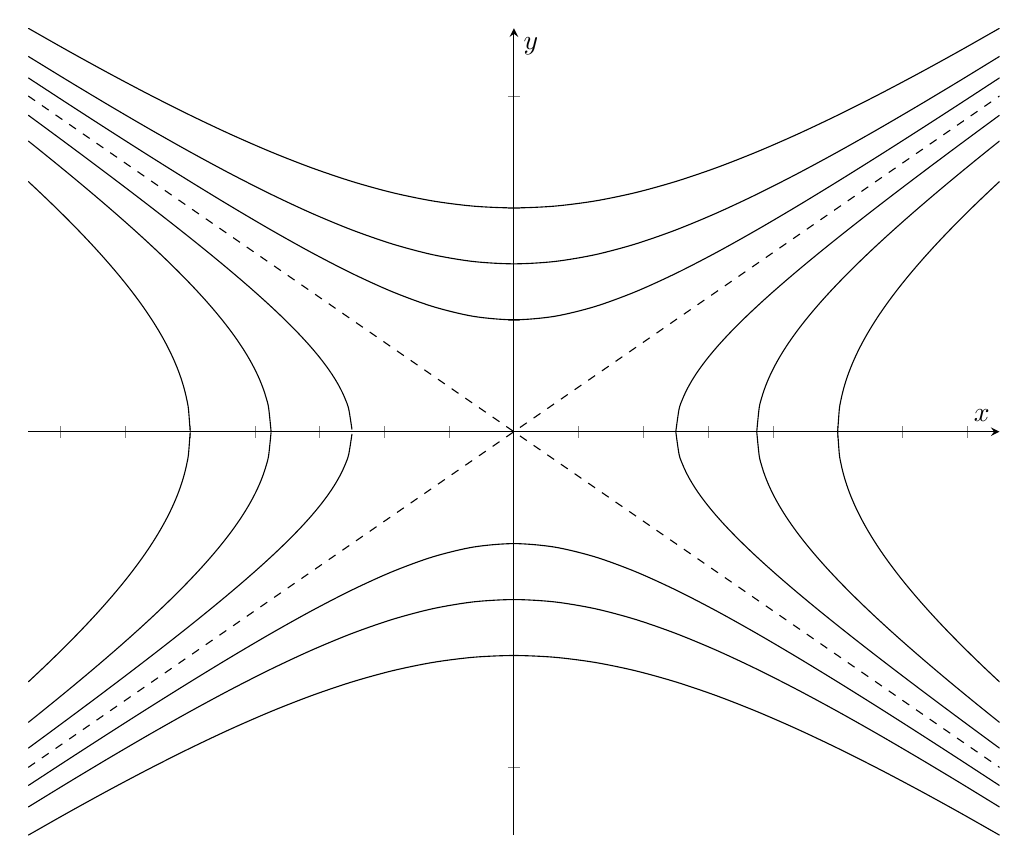
\begin{tikzpicture}
            \begin{axis} [
                scale=1.8,
                axis lines=center,
                xlabel={\(x\)},
                ylabel={\(y\)},
                xtick={},
                xticklabels={},
                ytick={},
                yticklabels={}]

                \addplot [domain=-1.5:1.5, smooth, dashed] { x };
                \addplot [domain=-1.5:1.5, smooth, dashed] { -x };

                \addplot [domain=-1.5:1.5, smooth] { sqrt(1 + x^2) };
                \addplot [domain=-1.5:1.5, smooth] { -sqrt(1 + x^2) };

                \addplot [domain=-1.5:1.5, smooth] { sqrt(0.75^2 + x^2) };
                \addplot [domain=-1.5:1.5, smooth] { -sqrt(0.75^2 + x^2) };

                \addplot [domain=-1.5:1.5, smooth] { sqrt(0.25 + x^2) };
                \addplot [domain=-1.5:1.5, smooth] { -sqrt(0.25 + x^2) };

                \addplot [domain=-1.5:-1, smooth, samples=100] { sqrt(-1 + x^2) };
                \addplot [domain=1:1.5, smooth, samples=100] { sqrt(-1 + x^2) };
                \addplot [domain=-1.5:-1, smooth, samples=100] { -sqrt(-1 + x^2) };
                \addplot [domain=1:1.5, smooth, samples=100] { -sqrt(-1 + x^2) };

                \addplot [domain=-1.5:-0.75, smooth, samples=100] { sqrt(-0.75^2 + x^2) };
                \addplot [domain=0.75:1.5, smooth, samples=100] { sqrt(-0.75^2 + x^2) };
                \addplot [domain=-1.5:-0.75, smooth, samples=100] { -sqrt(-0.75^2 + x^2) };
                \addplot [domain=0.75:1.5, smooth, samples=100] { -sqrt(-0.75^2 + x^2) };

                \addplot [domain=-1.5:-0.5, smooth, samples=100] { sqrt(-0.5^2 + x^2) };
                \addplot [domain=0.5:1.5, smooth, samples=100] { sqrt(-0.5^2 + x^2) };
                \addplot [domain=-1.5:-0.5, smooth, samples=100] { -sqrt(-0.5^2 + x^2) };
                \addplot [domain=0.5:1.5, smooth, samples=100] { -sqrt(-0.5^2 + x^2) };

            \end{axis}
        \end{tikzpicture}
    \end{center}

    Under the transformation \(y = \ln u - x\), the line \(y = x\) gets mapped to \(u = e^{2x}\), and the line \(y = -x\) gets mapped to \(u = 1\)

    \begin{center}
        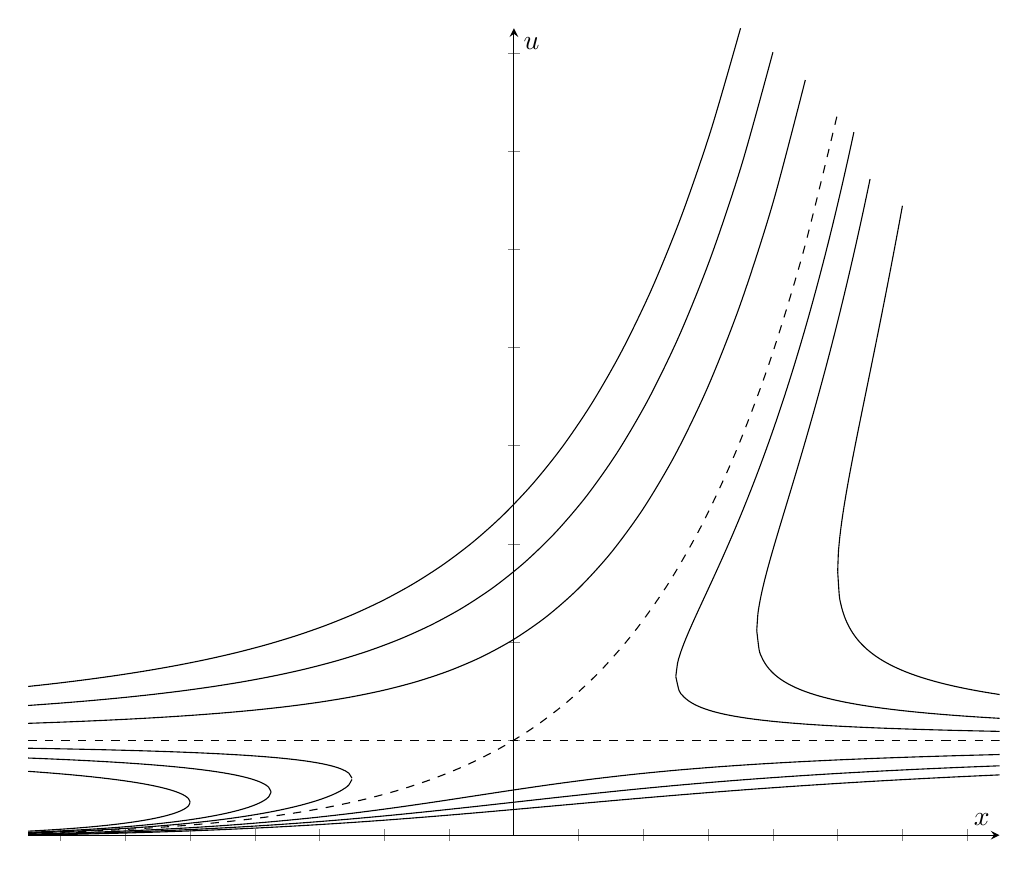
\begin{tikzpicture}
            \begin{axis} [
                scale=1.8,
                axis lines=center,
                xlabel={\(x\)},
                ylabel={\(u\)},
                xtick={},
                xticklabels={},
                ytick={},
                yticklabels={}]

                \addplot [domain=-1.5:1, smooth, dashed] { exp(2 * x) };
                \addplot [domain=-1.5:1.5, smooth, dashed] { 1 };

                \addplot [domain=-1.5:0.7, smooth] { exp(x + sqrt(x^2 + 1.5)) };
                \addplot [domain=-1.5:1.5, smooth] { exp(x - sqrt(x^2 + 1.5)) };

                \addplot [domain=-1.5:0.8, smooth] { exp(x + sqrt(x^2 + 1)) };
                \addplot [domain=-1.5:1.5, smooth] { exp(x - sqrt(x^2 + 1)) };

                \addplot [domain=-1.5:0.9, smooth] { exp(x + sqrt(x^2 + 0.5)) };
                \addplot [domain=-1.5:1.5, smooth] { exp(x - sqrt(x^2 + 0.5)) };

                \addplot [domain=1:1.2, smooth, samples=100] { exp(x + sqrt(x^2 - 1^2)) };
                \addplot [domain=-1.5:-1, smooth, samples=100] { exp(x + sqrt(x^2 - 1^2)) };
                \addplot [domain=1:1.5, smooth, samples=100] { exp(x - sqrt(x^2 - 1^2)) };
                \addplot [domain=-1.5:-1, smooth, samples=100] { exp(x - sqrt(x^2 - 1^2)) };

                \addplot [domain=0.75:1.1, smooth, samples=100] { exp(x + sqrt(x^2 - 0.75^2)) };
                \addplot [domain=-1.5:-0.75, smooth, samples=100] { exp(x + sqrt(x^2 - 0.75^2)) };
                \addplot [domain=0.75:1.5, smooth, samples=100] { exp(x - sqrt(x^2 - 0.75^2)) };
                \addplot [domain=-1.5:-0.75, smooth, samples=100] { exp(x - sqrt(x^2 - 0.75^2)) };

                \addplot [domain=0.5:1.05, smooth, samples=100] { exp(x + sqrt(x^2 - 0.5^2)) };
                \addplot [domain=-1.5:-0.5, smooth, samples=100] { exp(x + sqrt(x^2 - 0.5^2)) };
                \addplot [domain=0.5:1.5, smooth, samples=100] { exp(x - sqrt(x^2 - 0.5^2)) };
                \addplot [domain=-1.5:-0.5, smooth, samples=100] { exp(x - sqrt(x^2 - 0.5^2)) };
            \end{axis}
        \end{tikzpicture}
    \end{center}

\end{solution}

\begin{problem}
    Sketch the solution curves to the differential equation \(y' = \para{y + 1} y \para{y - 1}\). Sketch the solution curves to the differential equation \(y' = \para{y + 1}^2 y \para{y - 1}^2\). It would be helpful considering constant solutions in both cases, since solutions to differential equations cannot cross.
\end{problem}

\begin{solution}
    Let \(f\para{y} = \para{y + 1} y \para{y - 1}\). We first sketch the graph of \(f\para{y}\).

    \begin{center}
        \begin{tikzpicture}
            \begin{axis} [
                scale=1.8,
                axis lines=center,
                xlabel={\(y\)},
                ylabel={\(f\para{y}\)}]
                \addplot [domain=-1.5:1.5, smooth] { (x + 1) * x * (x - 1) };
            \end{axis}
        \end{tikzpicture}
    \end{center}

    Therefore, constant solutions of \(y\) are \(y = 0, \pm 1\), and \(y\) is increasing if \(-1 < y < 0\) or \(y > 1\), and \(y\) is decreasing if \(0 < y < 1\) or \(y < -1\).

    \begin{center}
        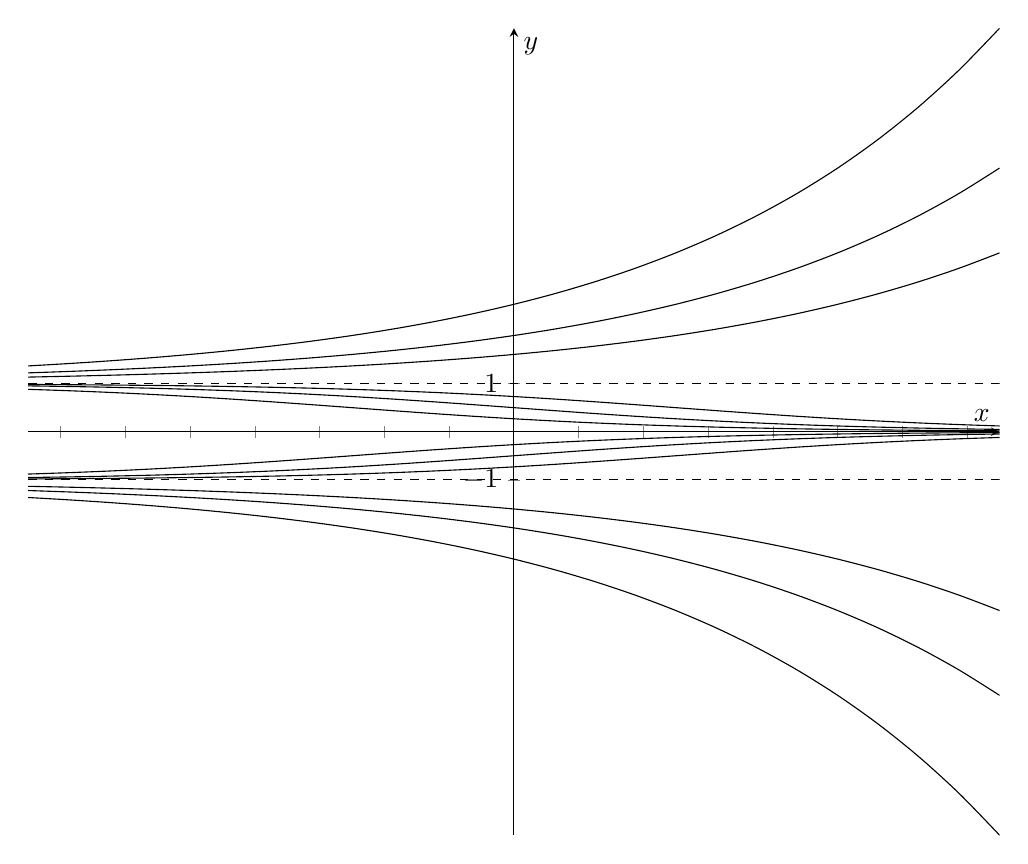
\begin{tikzpicture}
            \begin{axis} [
                scale=1.8,
                axis lines=center,
                xlabel={\(x\)},
                ylabel={\(y\)},
                xtick={},
                xticklabels={},
                ytick={-1, 1},
                yticklabels={\(-1\), \(1\)}]
                \addplot [domain=-1.5:1.5, smooth, dashed] { 1 };
                \addplot [domain=-1.5:1.5, smooth, dashed] { -1 };

                \addplot [domain=-1.5:1.5, smooth] { 1 + exp(x - 0.5) };
                \addplot [domain=-1.5:1.5, smooth] { 1 + exp(x) };
                \addplot [domain=-1.5:1.5, smooth] { 1 + exp(x + 0.5) };

                \addplot [domain=-1.5:1.5, smooth] { -0.5 * tanh(x - 0.5) + 0.5 };
                \addplot [domain=-1.5:1.5, smooth] { -0.5 * tanh(x) + 0.5 };
                \addplot [domain=-1.5:1.5, smooth] { -0.5 * tanh(x + 0.5) + 0.5 };

                \addplot [domain=-1.5:1.5, smooth] { 0.5 * tanh(x - 0.5) - 0.5 };
                \addplot [domain=-1.5:1.5, smooth] { 0.5 * tanh(x) - 0.5 };
                \addplot [domain=-1.5:1.5, smooth] { 0.5 * tanh(x + 0.5) - 0.5 };

                \addplot [domain=-1.5:1.5, smooth] { -1 - exp(x - 0.5) };
                \addplot [domain=-1.5:1.5, smooth] { -1 - exp(x) };
                \addplot [domain=-1.5:1.5, smooth] { -1 - exp(x + 0.5) };
            \end{axis}
        \end{tikzpicture}
    \end{center}

    Let \(g\para{y} = \para{y + 1}^2 y \para{y - 1}^2\). We first sketch the graph of \(g\para{y}\).

    \begin{center}
        \begin{tikzpicture}
            \begin{axis} [
                scale=1.8,
                axis lines=center,
                xlabel={\(y\)},
                ylabel={\(g\para{y}\)}]
                \addplot [domain=-1.5:1.5, smooth] { (x + 1) * (x + 1) * x * (x - 1) * (x - 1)};
            \end{axis}
        \end{tikzpicture}
    \end{center}

    Therefore, constant solutions are the same, but \(y\) is increasing for \(0 < y < 1\) or \(y > 1\), and \(y\) is decreasing if \(-1 < y < 0\) or \(y < -1\).

        \begin{center}
        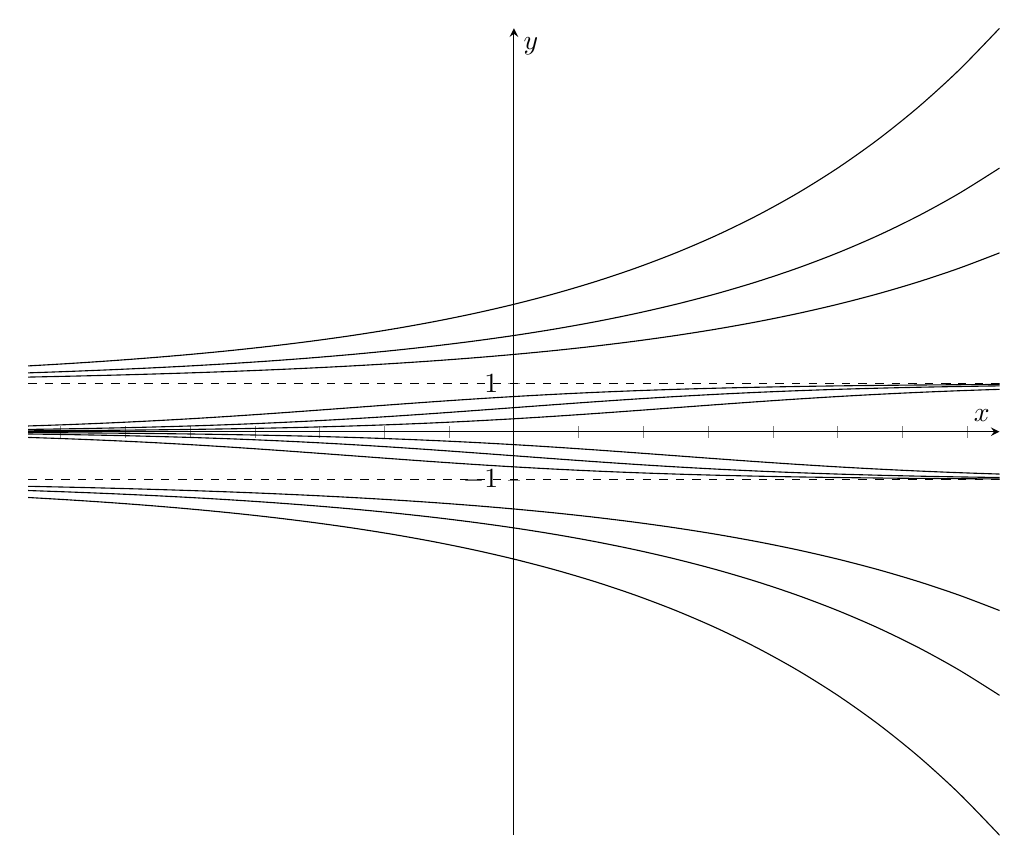
\begin{tikzpicture}
            \begin{axis} [
                scale=1.8,
                axis lines=center,
                xlabel={\(x\)},
                ylabel={\(y\)},
                xtick={},
                xticklabels={},
                ytick={-1, 1},
                yticklabels={\(-1\), \(1\)}]
                \addplot [domain=-1.5:1.5, smooth, dashed] { 1 };
                \addplot [domain=-1.5:1.5, smooth, dashed] { -1 };

                \addplot [domain=-1.5:1.5, smooth] { 1 + exp(x - 0.5) };
                \addplot [domain=-1.5:1.5, smooth] { 1 + exp(x) };
                \addplot [domain=-1.5:1.5, smooth] { 1 + exp(x + 0.5) };

                \addplot [domain=-1.5:1.5, smooth] { 0.5 * tanh(x - 0.5) + 0.5 };
                \addplot [domain=-1.5:1.5, smooth] { 0.5 * tanh(x) + 0.5 };
                \addplot [domain=-1.5:1.5, smooth] { 0.5 * tanh(x + 0.5) + 0.5 };

                \addplot [domain=-1.5:1.5, smooth] { -0.5 * tanh(x - 0.5) - 0.5 };
                \addplot [domain=-1.5:1.5, smooth] { -0.5 * tanh(x) - 0.5 };
                \addplot [domain=-1.5:1.5, smooth] { -0.5 * tanh(x + 0.5) - 0.5 };

                \addplot [domain=-1.5:1.5, smooth] { -1 - exp(x - 0.5) };
                \addplot [domain=-1.5:1.5, smooth] { -1 - exp(x) };
                \addplot [domain=-1.5:1.5, smooth] { -1 - exp(x + 0.5) };
            \end{axis}
        \end{tikzpicture}
    \end{center}
\end{solution}